\documentclass{article}

\usepackage{amsmath,amssymb}
\usepackage{tikz}
\usepackage{pgfplots}
\usetikzlibrary{intersections}
\usepgfplotslibrary{fillbetween}
\usepackage{xcolor}
\usepackage[left=2.1cm,right=3.1cm,bottom=3cm,footskip=0.75cm,headsep=0.5cm]{geometry}
\usepackage{enumerate}
\usepackage{enumitem}
\usepackage{marvosym}
\usepackage{tabularx}
\usepackage{parskip}

\usepackage{listings}
\definecolor{lightlightgray}{rgb}{0.95,0.95,0.95}
\definecolor{lila}{rgb}{0.8,0,0.8}
\definecolor{mygray}{rgb}{0.5,0.5,0.5}
\definecolor{mygreen}{rgb}{0,0.8,0.26}
\lstdefinestyle{R} {language=R,morekeywords={confint,head,fitdist,ks,test}}
\lstset{language=R,
	basicstyle=\ttfamily,
	keywordstyle=\color{lila},
	commentstyle=\color{lightgray},
	stringstyle=\color{mygreen}\ttfamily,
	backgroundcolor=\color{white},
	showstringspaces=false,
	numbers=left,
	numbersep=10pt,
	numberstyle=\color{mygray}\ttfamily,
	identifierstyle=\color{blue},
	xleftmargin=.1\textwidth, 
	%xrightmargin=.1\textwidth,
	escapechar=§,
}
\usepackage[colorlinks = true, linkcolor = blue, urlcolor  = blue, citecolor = blue, anchorcolor = blue]{hyperref}

\usepackage[utf8]{inputenc}
\usepackage[onehalfspacing]{setspace}

\renewcommand*{\arraystretch}{1.4}

\newcolumntype{L}[1]{>{\raggedright\arraybackslash}p{#1}}
\newcolumntype{R}[1]{>{\raggedleft\arraybackslash}p{#1}}
\newcolumntype{C}[1]{>{\centering\let\newline\\\arraybackslash\hspace{0pt}}m{#1}}

\newcommand{\E}{\mathbb{E}}
\DeclareMathOperator{\Var}{Var}
\DeclareMathOperator{\CDF}{CDF}

\title{\textbf{Wie funktionieren statistische Tests?}}
\author{\textsc{Henry Haustein}}
\date{}

\begin{document}
	\maketitle
	
	In den letzten Jahren sind rund 35\% der Studenten durch die Statistik-Prüfung gefallen. Während Corona sank diese Quote auf rund 15\%. Ist diese Änderung zufällig oder war das Online-Lehre des Lehrstuhls so gut, dass plötzlich so viele Studenten die Inhalte verstanden haben\footnote{Betrug während der Klausur ist natürlich völlig ausgeschlossen...}?
	
	Genau solche Fragen können statistische Tests beantworten. Wir brauchen dazu
	\begin{itemize}
		\item 2 Hypothesen, die sich gegenseitig ausschließen
		\item eine Teststatistik
		\item einen kritischen Wert
	\end{itemize}

	Die Hypothesen dienen dazu, den Test zu formalisieren und sich bewusst zu machen, was man eigentlich testen möchte. Durch eine sprachliche Beschreibung ist dies nicht immer präzise möglich. Aufgrund der stochastischen Hintergründe eines Tests kann man die Nullhypothese nur annehmen oder nicht annehmen (aber nicht ablehnen!), weswegen man die zu testende Aussage immer als Alternativhypothese auffasst (\textit{Testen Sie, ob er Mittelwert kleiner als 15 ist!} $\Rightarrow$ $H_1: \mu < 15$ und damit $H_0: \mu \ge 15$). Sollen wir auf Gleichheit testen, so ist Gleichheit immer in der Nullhypothese und die Ungleichheit immer in der Alternativhypothese. \\
	Im obigen Beispiel wollen wir ja testen, ob bei einer Durchfallquote von 35\% es sein kann, dass nur 15\% durchgefallen sind. Ist also die Durchfallquote nur 15\%? Die Hypothesen sind also
	\begin{align}
		H_0: \hat{p} &= 0.15 \notag \\
		H_1: \hat{p} &\neq 0.15 \notag
	\end{align}
	
	Die Teststatistik hängt vom Test ab, der durchgeführt werden soll und steht immer in der Formelsammlung. Für unser Beispiel oben ist die Teststatistik (ich habe einfach mal $n=400$ angenommen)
	\begin{align}
		T &= \frac{\hat{p} - p}{\sqrt{\frac{p(1-p)}{n}}} \notag \\
		&= \frac{0.15-0.35}{\sqrt{\frac{0.35\cdot 0.65}{400}}} \notag \\
		&= -8.3863 \notag
	\end{align}
	Welche Bedeutung hat die Teststatistik? Sie ist ein Maß für den Abstand zwischen dem, was wir erwarten (35\% Durchfallquote) und dem, was wir beobachten (15\% Durchfallquote). Eine sehr hohe oder sehr niedrige Teststatistik deutet also darauf hin, dass Erwartung und Beobachtung auseinander fallen und ist damit ein Zeichen dafür, dass die Nullhypothese zweifelhaft ist. \\
	Aber warum ist dann die Berechnung der Teststatistik so kompliziert? Die Teststatistik
	\begin{align}
		\tilde{T} &= \hat{p} - p \notag \\
		&= 0.15 - 0.35 \notag \\
		&= -0.2 \notag
	\end{align}
	ist ja auch ein Maß für den Abstand zwischen Erwartung und Beobachtung. \\
	Das hat mit den kritischen Werten zu tun. Die Teststatistik $T$ hat die weitere Eigenschaft, dass sie approximativ standardnormalverteilt ist. Diese Eigenschaft brauchen wir, wenn wir die kritischen Werte einfach und schnell ermitteln wollen. Deren Berechnung ist noch viel komplizierter\footnote{Hier muss man Integrale berechnen, die keine Stammfunktion haben und häufig braucht man noch die Gamma-Funktion. Beides sind Rechenoperationen, die heutzutage nur effizient ein Computer lösen machen kann, aber als diese Tests entwickelt wurden gab es noch keine Computer und die Berechnung war sehr aufwendig. Die kritischen Werte wurden dann nur einmal berechnet und die Ergebnisse wurden weitergegeben. Klar, dass man lieber eine etwas aufwendigere Teststatistik berechnet als die kritischen Werte jedes mal neu zu bestimmen.}, aber sie hängen (fast) nicht mehr von den Parametern des Tests ab.
	
	Welche Rolle spielen die kritischen Werte? Sie geben die Grenze an, bis wann eine Abweichung vom Erwarteten noch ok ist. Die unsere Teststatistik ist approximativ standardnormalverteilt, also
	\begin{center}
		\begin{tikzpicture}
			\begin{axis}[
				xmin=-3, xmax=3, xlabel={$T$},
				ymin=0, ymax=0.5,
				samples=400,
				axis x line=middle,
				axis y line=middle,
				domain=-3:3,
				]
				\addplot[blue] {1/sqrt(2*pi) * exp(-0.5*x*x)};
				
			\end{axis}
		\end{tikzpicture}
	\end{center}
	Bei einem Test brauchen wir auch immer eine Irrtumswahrscheinlichkeit $\alpha$. Sie gibt an, wie stark wir Abweichungen vom Erwarteten tolerieren. $\alpha$ heißt deswegen Irrtumswahrscheinlichkeit, weil es angibt, wie wahrscheinlich es ist, dass die Abweichung so groß ist, dass wir sie nicht mehr tolerieren, aber das Erwartete immer noch stimmt.
	\begin{center}
		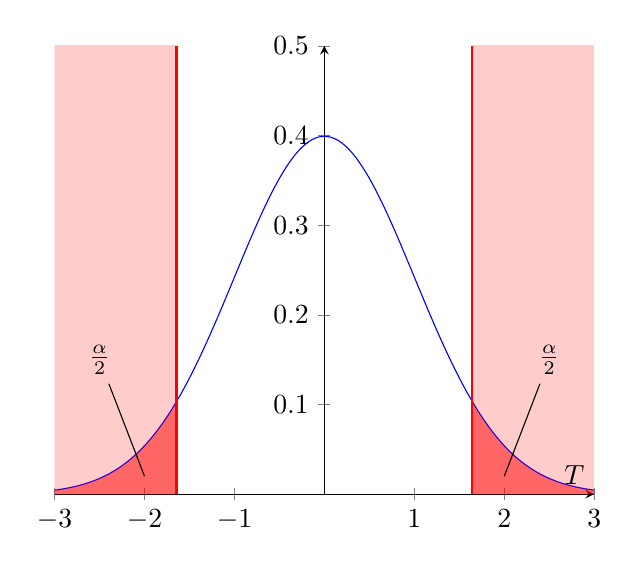
\begin{tikzpicture}
			\begin{axis}[
				xmin=-3, xmax=3, xlabel={$T$},
				ymin=0, ymax=0.5,
				samples=400,
				axis x line=middle,
				axis y line=middle,
				domain=-3:3,
				]
				\addplot[blue, name path=A] {1/sqrt(2*pi) * exp(-0.5*x*x)};
				\addplot[black, name path=B] {0};
				\addplot [red, opacity=0.5] fill between [of = A and B, soft clip={domain=-3:-1.6449}];
				\addplot [red, opacity=0.5] fill between [of = A and B, soft clip={domain=1.6449:3}];
				\draw[red,thick] (axis cs: -1.6449,0) -- (axis cs: -1.6449,0.5);
				\draw[red,thick] (axis cs: 1.6449,0) -- (axis cs: 1.6449,0.5);
				\draw[red,fill=red,opacity=0.2] (axis cs: -3,0) rectangle (axis cs: -1.6449,0.5);
				\draw[red,fill=red,opacity=0.2] (axis cs: 3,0) rectangle (axis cs: 1.6449,0.5);
				
				\node at (axis cs: -2.5,0.15) (a) {$\frac{\alpha}{2}$};
				\draw (a) -- (axis cs: -2,0.02);
				\node at (axis cs: 2.5,0.15) (b) {$\frac{\alpha}{2}$};
				\draw (b) -- (axis cs: 2,0.02);
			\end{axis}
		\end{tikzpicture} \\
		Die Grafik ist für einen zweiseitigen Test. Es gibt auch einseitige Tests, aber da ist der Ablehnungsbereich nur entweder links oder rechts, die Grenzen sind damit andere. Sonst ändert sich nichts, weswegen ich im Folgenden immer von zweiseitigen Tests ausgehen werde.
	\end{center}
	Der rote Bereich ist der Ablehnungsbereich, das heißt sollte die Teststatistik einen Wert annehmen, der in diesem Bereich liegt, so nimmt man $H_0$ nicht an, sondern entscheidet sich für die Alternativhypothese. Der Ablehnungsbereich ist so konstruiert, dass die Fläche unter der Verteilung der Teststatistik im Ablehnungsbereich genau $\alpha$ ist. Die Grenzen des Ablehnungsbereiches sind die kritischen Werte. \\
	Für unser Beispiel bedeutet dies, dass das Bild so aussieht (mit $\alpha =10\%$ ergeben sich die kritischen Werte zu $\pm 1.6449$):
	\begin{center}
		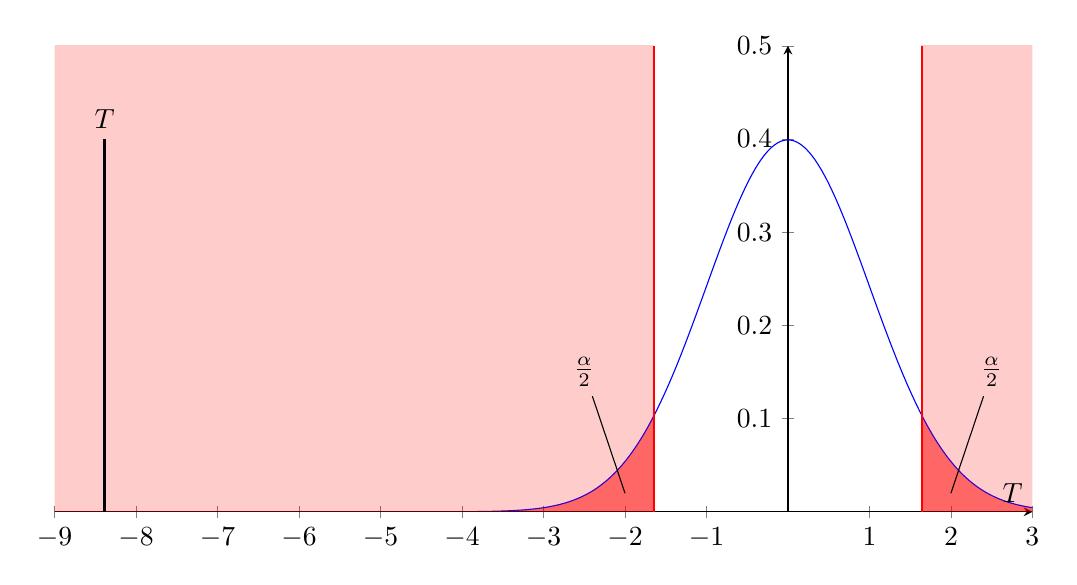
\begin{tikzpicture}
			\begin{axis}[
				xmin=-9, xmax=3, xlabel={$T$},
				ymin=0, ymax=0.5,
				samples=400,
				axis x line=middle,
				axis y line=middle,
				domain=-9:3,
				width=14cm,
				height=7.5cm
				]
				\addplot[blue, name path=A] {1/sqrt(2*pi) * exp(-0.5*x*x)};
				\addplot[black, name path=B] {0};
				\addplot [red, opacity=0.5] fill between [of = A and B, soft clip={domain=-9:-1.6449}];
				\addplot [red, opacity=0.5] fill between [of = A and B, soft clip={domain=1.6449:3}];
				\draw[red,thick] (axis cs: -1.6449,0) -- (axis cs: -1.6449,0.5);
				\draw[red,thick] (axis cs: 1.6449,0) -- (axis cs: 1.6449,0.5);
				\draw[red,fill=red,opacity=0.2] (axis cs: -9,0) rectangle (axis cs: -1.6449,0.5);
				\draw[red,fill=red,opacity=0.2] (axis cs: 3,0) rectangle (axis cs: 1.6449,0.5);
				
				\node at (axis cs: -2.5,0.15) (a) {$\frac{\alpha}{2}$};
				\draw (a) -- (axis cs: -2,0.02);
				\node at (axis cs: 2.5,0.15) (b) {$\frac{\alpha}{2}$};
				\draw (b) -- (axis cs: 2,0.02);
				
				\draw[black, thick] (axis cs: -8.3863, 0) -- (axis cs: -8.3863, 0.4) node[above] {$T$};
			\end{axis}
		\end{tikzpicture}
	\end{center}
	Unsere Teststatistik $T$ ist im Ablehnungsbereich, wir nehmen also $H_0$ nicht an und entscheiden uns für $H_1$.
	
	Besonders im angelsächsichen Raum wird häufig nicht mit kritischen Werten, sondern mit p-values gearbeitet. Das ist die Fläche unter der Dichtefunktion bis zur Teststatistik $T$:
	\begin{center}
		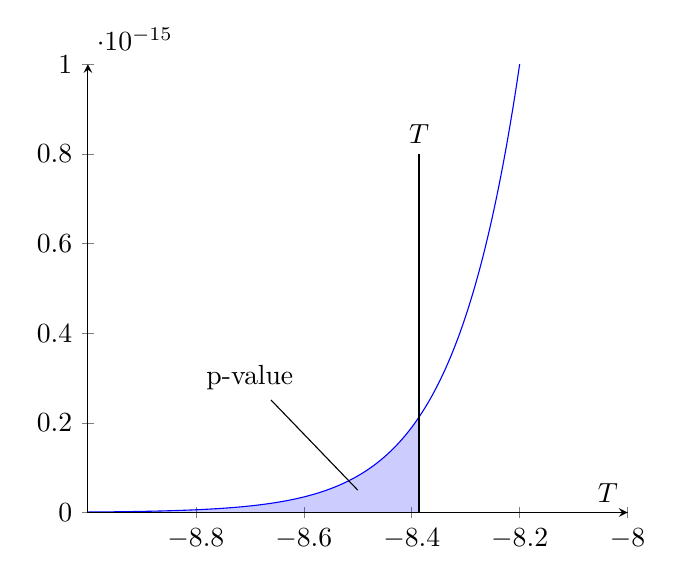
\begin{tikzpicture}
			\begin{axis}[
				xmin=-9, xmax=-8, xlabel={$T$},
				ymin=0, ymax=0.000000000000001,
				samples=400,
				axis x line=middle,
				axis y line=left,
				domain=-9:-8,
				]
				\addplot[blue, name path=A] {1/sqrt(2*pi) * exp(-0.5*x*x)};
				\addplot[black, name path=B] {0};
				\addplot [blue, opacity=0.2] fill between [of = A and B, soft clip={domain=-9:-8.3863}];
				
				\draw[black, thick] (axis cs: -8.3863, 0) -- (axis cs: -8.3863, 0.0000000000000008) node[above] {$T$};
				
				\node at (axis cs: -8.7,0.0000000000000003) (a) {p-value};
				\draw (a) -- (axis cs: -8.5,0.00000000000000005);
			\end{axis}
		\end{tikzpicture}
	\end{center}
	In unserem Beispiel beträgt dieser $\Phi(-8.3863) = 2.50841\cdot 10^{-17}$. Sind die p-values sehr klein, so liegt $T$ weit weg vom Erwarteten und damit säht das Zweifel an $H_0$. Hat eine Teststatistik einen p-value von $>\frac{\alpha}{2}$, so liegt $T$ im Nicht-Ablehnungsbereich und damit wird $H_0$ angenommen.
	
	\section*{Zusammenhang mit Konfidenzintervallen}
	
	Statistische Tests und Konfidenzintervalle hängen stark zusammen und die Aussage, die sie machen, ist die selbe. Man könnte den Nicht-Ablehnungsbereich als Konfidenzintervall für die Teststatistik bezeichnen. Falls die Teststatistik in dieses Konfidenzintervall fällt, so wird $H_0$ angenommen.
	
\end{document}